% Working manuscript, refined 2026-10-22. Author metadata is intentionally omitted.
\documentclass[sigconf,10pt]{acmart}
\setcopyright{none}
\settopmatter{printacmref=false,printfolios=true}
\renewcommand\footnotetextcopyrightpermission[1]{}
\acmConference[MobiSys working draft]{MobiSys working draft}{}{}
\acmDOI{}
\acmISBN{}
\usepackage{booktabs}
\usepackage{tabularx}
\renewcommand{\shortauthors}{}
\begin{document}
\title{Policy-Aligned Feature Streaming for Efficient Edge--Cloud VLA Inference}
\begin{abstract}
Edge--cloud vision--language--action (VLA) inference must balance control
quality, visual communication cost, and computation on the robot and
server. Image compression reduces traffic but leaves image decoding and
visual encoding in the cloud; moving the full visual encoder to the robot
can instead make local computation expensive. We present a
feature-streaming interface that combines a distilled edge visual tower,
a learned codec, and direct recovery of a frozen policy's visual tokens.
The original policy's clean-input actions and tokens supervise training
alongside a rate objective. Temporal prediction uses quantized code
references without a neural decoder on the robot, and integer rANS
produces the transmitted bitstream.
We implement the design for $\pi_{0.5}$ and adapt its visual interface to
OpenVLA-OFT. In 2,000 paired LIBERO episodes, the primary configuration
achieves 96.7\% success versus 96.9\% for the reference, with a paired
difference of $-0.20$ percentage points and a 95\% confidence interval of
$[-1.21,0.81]$. A separate rANS deployment subset yields a mean sampled
payload of 1.82\,kB per upload. On recorded SO-101 observations replayed
through an Orin-to-A40 deployment, median end-to-end latency is
228.4\,ms versus 272.4\,ms for H.264 at a similar payload.
These results support the interface under the tested conditions but do
not establish physical closed-loop benefits, a complete cross-backbone
comparison, or robustness under distribution shift.
\end{abstract}
\keywords{Vision-language-action models, edge-cloud inference, feature compression, robotic systems}
\maketitle
\section{Introduction}
\label{sec:introduction}
\begin{figure}[t]
  \centering
  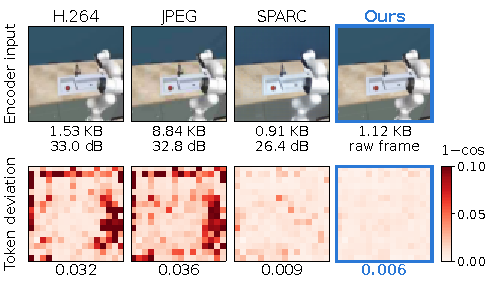
\includegraphics[width=\columnwidth]{images/pixel-vs-control.pdf}
  \caption{Pixel fidelity is not control fidelity. On RoboCasa, H.264
  frames at 3.0\,KB per upload look close to the originals, yet
  $\pi_{0.5}$ succeeds in 0 of 480 episodes; the policy tokens computed
  from them deviate most around the robot arm. Our frontend sends
  1.14\,KB per upload, recovers tokens close to the clean ones, and
  succeeds in 295 of 480 episodes (uncompressed: 291). Deviation is
  $1-\cos$ between each post-projection policy token and its clean
  counterpart, overlaid on a lightened copy of the original frame. The
  upload shown has the median H.264 deviation in its episode; across all
  24 uploads and three cameras of that episode, H.264 deviation averages
  $4.0\times$ ours.}
  \Description{Four square panels of a simulated kitchen with a robot arm.
  The original frame and the H.264 frame look almost identical. A heatmap
  of token deviation for H.264 is bright around the robot arm and at some
  image borders, with mean 0.032. The same heatmap for our frontend is
  almost dark, with mean 0.006.}
  \label{fig:pixel-vs-control}
\end{figure}
% TODO(author): replace the single-episode ratio (4.0x) with the held-out
% 8-episode average once computed.

A robot using a remotely hosted vision--language--action (VLA) policy must
repeatedly send visual observations and receive actions while its physical
state continues to change. Models such as $\pi_{0.5}$ and OpenVLA use
visual observations and language to support manipulation
tasks~\cite{pi05,openvla}. OpenVLA-OFT studies how adaptation and action
decoding affect both speed and success~\cite{openvlaoft}. In an edge--cloud
deployment, these capabilities depend on more than policy inference
alone. The robot must prepare its observations, transfer them, and wait
for the cloud to process them. Our SO-101 deployment makes this division
concrete: an Orin device processes camera inputs while an A40 server
hosts the policy. Work added to either side recurs with each new visual
request.

Image offloading and model partitioning address different parts of this
cost. Progressive image transmission, exemplified by LimitNet, targets
vision offloading under constrained device and network
resources~\cite{limitnet}. SPARC goes further for VLA policies by using
action-aware image compression and temporal masking~\cite{sparc}.
These approaches still recover images before the policy's visual
processing. Image fidelity, however, is a poor proxy for what the policy needs:
H.264 frames that look nearly unchanged can make the policy fail in every
episode (Figure~\ref{fig:pixel-vs-control}). Collaborative inference systems instead choose where model
computation runs~\cite{neurosurgeon,roboecc,rapid}, while feature
communication methods such as BottleNet++ compress intermediate
representations~\cite{bottlenetpp}. For a robot, moving a full visual
encoder to the edge can trade network traffic for local computation.
Consequently, a smaller payload alone does not establish a faster
deployment, and the best division of work depends on the representation
that crosses the network.

We study a visual communication interface that recovers the tokens
consumed by a frozen VLA policy. A lightweight encoder on the robot
produces a discrete feature stream, and a cloud decoder supplies the
policy's visual inputs without reconstructing an intermediate image.
For our primary $\pi_{0.5}$ configuration, the receiver replaces the
original visual tower and projection. This choice changes both the
communication payload and the computation required to consume it. Our
goal is to make this interface useful on a constrained edge device while
limiting its effect on control quality. We evaluate it against the
original policy under the same task conditions rather than treating
differences between policy backbones as compression gains.

Three obstacles shape the design. First, feature similarity is an
incomplete proxy for action quality: a compact representation must retain
information needed by the downstream controller. Second, the edge encoder
must be cheap enough that its work does not erase savings in communication
or cloud processing. Third, temporal coding must keep the sender and
receiver consistent without requiring a neural reconstruction decoder on
the robot. These obstacles concern the representation, the local
computation, and the state carried across uploads. Measuring their
combined effect also requires distinguishing visual-path microbenchmarks,
complete request latency, and physical task outcomes.

Our design combines policy supervision, a distilled visual tower, and
temporal coding over quantized features. Clean-input tokens and actions
from the original policy supervise the trainable student and codec while
the policy weights stay frozen. A compact student reduces visual
encoding work relative to running the original tower on the robot,
following the use of teacher supervision
for model compression~\cite{distillation}. Quantized code references
support temporal prediction, and integer rANS turns the resulting symbols
into a deployable bitstream~\cite{ans}. The cloud reconstructs policy
tokens directly. We implement the main path for $\pi_{0.5}$ and adapt
the student and decoder interface to OpenVLA-OFT. Each policy requires
its own training; the design does not assume that a single codec can
serve arbitrary VLA backbones.

This paper contributes a policy-aligned feature interface and its
training design (\S\ref{sec:overview}--\S\ref{sec:design-objective}), a
temporal bitstream implementation that avoids neural decoding at the
edge (\S\ref{sec:design-temporal}--\S\ref{sec:implementation}), and an
empirical characterization of the quality--cost tradeoff
(\S\ref{sec:evaluation}). The current evidence includes paired simulation
results and recorded-observation replay through a real edge--cloud stack.
It also identifies limits: the confidence intervals do not establish
lossless control, SPARC can use fewer bytes, stronger cloud hardware can
reduce the latency advantage, and shifted visual conditions can lower
success. These boundaries motivate evaluating a communication interface
as part of a control system rather than ranking codecs by payload alone.

\section{Background and Motivation}
\label{sec:background}
\subsection{The Observation--Action Loop}
A VLA policy consumes images, a language instruction, and any required
robot state, and returns actions. In a policy that uses action chunks,
one request produces several future control steps; OpenVLA-OFT explicitly
uses action chunking in its fine-tuning recipe~\cite{openvlaoft}. The
actuator control rate and the policy request rate therefore describe
different parts of the system. Increasing the former does not imply
that a fresh visual inference is performed at every control step.

This distinction matters when evaluating an edge--cloud path. An upload
can complete faster without improving a task if the returned action is
not needed immediately, or if errors in the visual representation impair
the next motion. Conversely, a delayed request can make its observation
stale by the time the action is used. TimelyLLM studies the relationship
between inference service and physical execution for agents~\cite{timelyllm}.
Here we focus on the representation sent with visual policy requests.
Our measured request latency ends when the action response returns; it
does not by itself measure observation age at physical action application.

\subsection{The Cost of Visual Communication}
\label{sec:bg-cost}
There are three relevant paths. Image offloading encodes pixels on the
edge and reconstructs them before cloud visual inference. Conventional
partitioning runs a model prefix locally and transmits intermediate
activations. Our path learns a compact representation and a receiver
that recovers policy input tokens. Table~\ref{tab:paths} summarizes these
interfaces. Model splitting and feature compression are established
ideas~\cite{neurosurgeon,bottlenetpp}; the question here is how to realize
the feature interface for a frozen VLA on robot hardware.

\begin{table}[t]
\caption{Visual communication interfaces. The policy after visual-token
construction is shared within each backbone comparison.}
\label{tab:paths}
\centering\small
\begin{tabularx}{\columnwidth}{lXX}
\toprule
Path & Transmitted representation & Cloud visual work \\
\midrule
Image codec & Image/video bitstream & Image decoding and original visual encoder \\
Model split & Intermediate activations & Remaining model computation \\
Feature streaming & Quantized feature bitstream & Feature recovery and token injection \\
\bottomrule
\end{tabularx}
\end{table}

The relevant cost includes edge preparation, transfer, and cloud
processing. A method with fewer bytes can still have a longer request
latency if encoding is expensive. A method with a more expensive encoder
can be useful if it removes sufficient receiver work. These alternatives
must be timed on the intended hardware. In particular, savings measured
on one cloud GPU need not persist on another.

\subsection{Why Policy Alignment Matters}
\label{sec:bg-align}
Image compression commonly trades rate against visual distortion;
learned hyperprior codecs provide one example of this
formulation~\cite{hyperprior}. A VLA introduces a different endpoint:
the recovered observation must support the action policy. SPARC addresses
this distinction with action distortion and a rate penalty
rather than relying on image fidelity alone~\cite{sparc}. Our design
retains the task-oriented endpoint while changing the receiver output
from pixels to policy tokens.

Our diagnostics also show that additional capacity or lower
feature error cannot be interpreted in isolation. Changing an input
preprocessing protocol changes the policy's reference performance, and
perturbed camera views can expose a quality loss that is small on the
original benchmark. We therefore report the input protocol, retain
negative results, and measure closed-loop simulation success separately
from feature reconstruction error and request latency.

\section{System Overview}
\label{sec:overview}

\begin{figure*}[t]
  \centering
  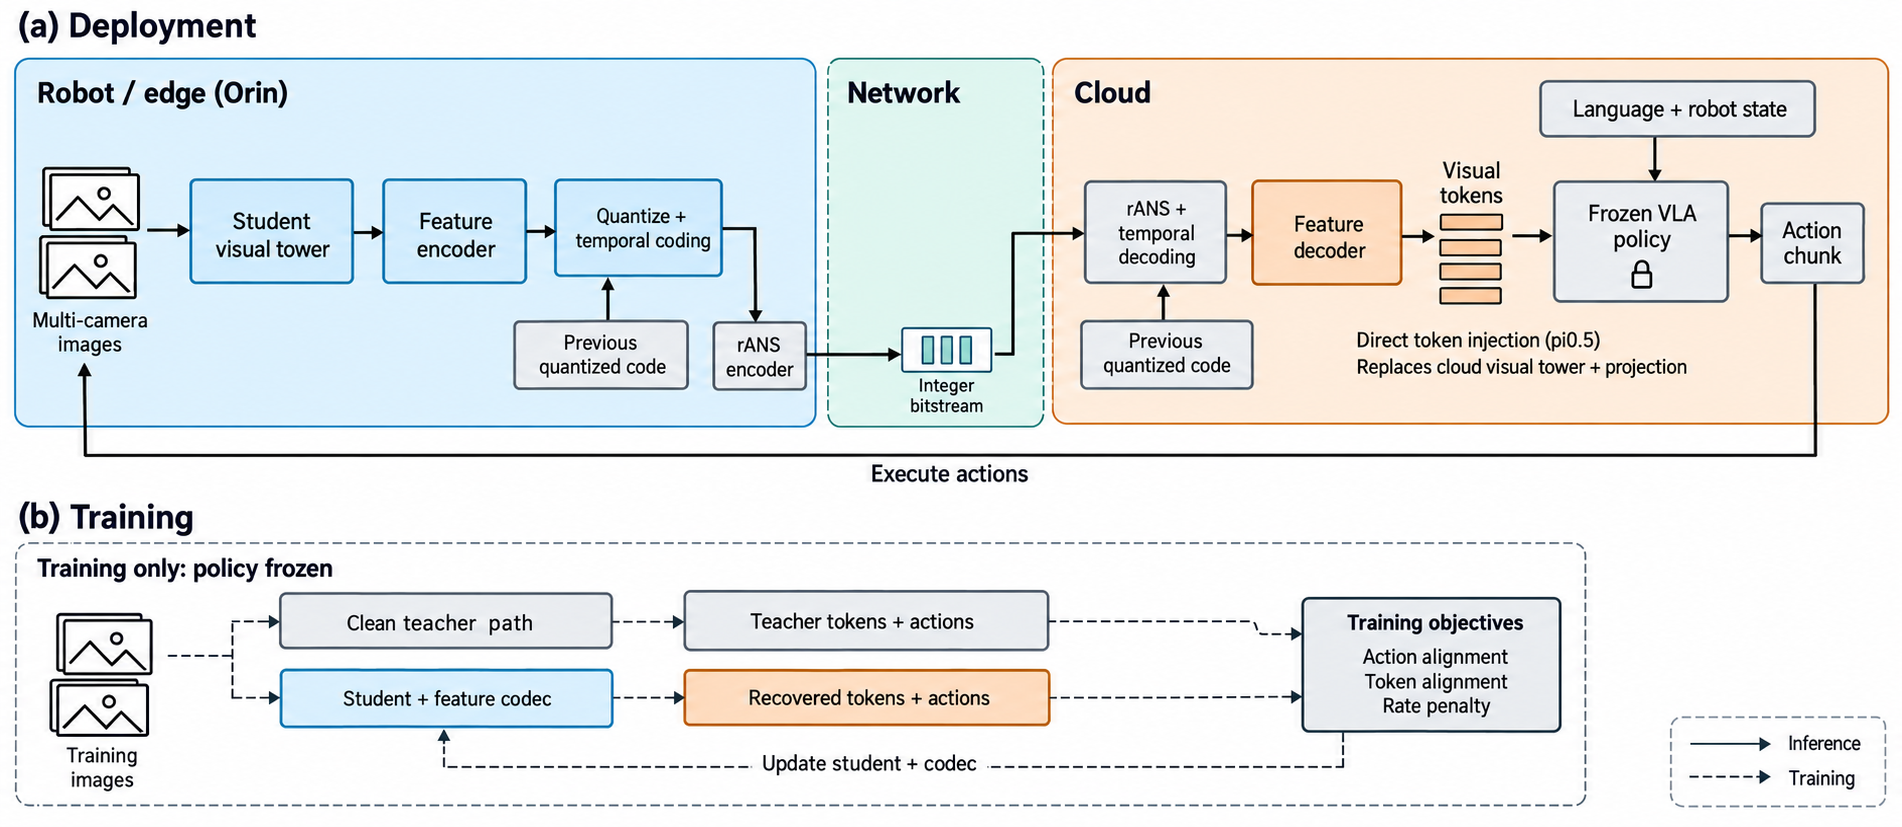
\includegraphics[width=\textwidth]{images/system-architecture-v1.png}
  \caption{System overview (primary $\pi_{0.5}$ configuration).
  (a) Deployment: the robot turns camera images into an integer bitstream;
  the cloud recovers the policy's visual tokens from the bitstream and runs
  the frozen VLA policy, skipping the cloud visual encoder.
  (b) Training: the student tower and codec are trained against the frozen
  policy's own tokens and actions on clean images, with a rate penalty.}
  \Description{Top panel: on the robot, multi-camera images pass through a
  student visual tower, feature encoder, quantization with temporal coding
  against the previous quantized code, and an rANS encoder; an integer
  bitstream crosses the network; in the cloud, rANS and temporal decoding,
  a feature decoder, and visual tokens feed a frozen VLA policy that also
  receives language and robot state and returns an action chunk. Bottom
  panel: a clean teacher path and the student-plus-codec path produce tokens
  and actions that supply action supervision, token alignment,
  and a rate penalty; only the student and codec are updated.}
  \label{fig:overview}
\end{figure*}

Each policy request incurs computation on the robot, transmission over the
network, and computation in the cloud~\cite{neurosurgeon,roboecc}.
Existing designs shift cost among the three (\S\ref{sec:bg-cost}). Image
codecs keep transmission small, but the cloud must still decode each image
and run the policy's visual encoder~\cite{limitnet,sparc}. Splitting the
policy can move that encoder onto the robot~\cite{roboecc}, where it
competes for limited compute. Our system transmits the policy's visual
features instead of images: it spends a small amount of computation on the
robot, sends a compact bitstream, and removes visual encoding from the
cloud for the primary configuration, while the policy weights stay unchanged.

\paragraph{Pipeline.}
Figure~\ref{fig:overview}a shows the deployed pipeline. On the robot, a
compact student tower distilled from the policy's visual encoder extracts
features from each camera image, and a feature encoder and quantizer map
them to integer codes. Each code is predicted from the code sent at the
previous upload, except at periodic intra frames, and the residual is
entropy-coded with integer rANS. In the cloud, the receiver reverses the
entropy and temporal coding to recover the codes exactly, and a feature
decoder turns them into visual tokens that replace the output of the
policy's visual encoder. The frozen policy consumes these tokens together
with the language instruction and robot state, which bypass the codec, and
returns an action chunk.

The design must solve four problems.

\paragraph{Preserving actions rather than appearance.}
Faithful reconstruction of images or features does not guarantee that the
policy acts the same (\S\ref{sec:bg-align}). We therefore supervise the
student tower and codec with the frozen policy's own outputs on clean
images. An action term supervises the frozen policy under recovered tokens
using clean-policy action targets, a token term aligns the tokens
themselves, and a rate term controls the coding budget
(Figure~\ref{fig:overview}b, \S\ref{sec:design-objective}).

\paragraph{Keeping robot computation small.}
Running the policy's visual encoder at every upload adds substantial
latency on resource-constrained robot hardware. The robot instead runs the
distilled student tower, trained jointly with the codec, so its work is
limited to the student tower, the feature encoder, and entropy coding
(\S\ref{sec:design-objective}).

\paragraph{Temporal coding without a decoder on the robot.}
Video codecs predict each frame from a reconstructed reference, so the
encoder also runs the decoder. For a learned codec, this would place a
neural decoder on the robot, and floating-point differences between the
robot and the cloud could desynchronize the reference. We instead predict
in the space of quantized codes, which both ends hold exactly, and use
integer-only rANS to produce identical bitstreams from the same symbols
and coding tables on ARM and x86 hosts
(\S\ref{sec:design-temporal}).

\paragraph{Adapting visual interfaces.}
Backbones consume visual features in different forms: $\pi_{0.5}$ takes
projected SigLIP tokens, whereas OpenVLA-OFT fuses features from two
visual towers. The pipeline structure is shared; the student tower and
feature decoder are adapted to each backbone's interface, and the codec is
trained once per backbone (\S\ref{sec:design-integration}).

\section{Design}
\label{sec:design}
\subsection{Policy-Aligned Compact Features}
\label{sec:design-objective}
The visual interface has a teacher path and a compressed student path
during training. The teacher uses the original visual encoder and frozen
policy on clean images to produce reference tokens and actions. The
student path replaces visual processing with a compact tower, feature
encoding, quantization, and feature decoding. Its recovered tokens enter
the same policy interface. The policy weights remain fixed, but gradients
propagate through the policy to update the trainable visual path.

The objective combines three terms. The action term penalizes changes in
policy behavior after compression. For $\pi_{0.5}$, training uses the
frozen policy's flow-matching objective with targets derived from its own
clean-input actions. For OpenVLA-OFT, the recorded action-distillation
configuration uses an L1 loss on clean-policy action chunks. The token
term aligns recovered tokens with the original visual representation
using mean-squared error and cosine similarity. The rate term penalizes
coding cost and is adjusted toward a target payload during
training. These terms respectively constrain the downstream behavior,
the intermediate representation, and the communication cost.

The clean actions in this procedure are outputs of the original policy,
not additional expert action annotations. Token supervision anchors the
student to the original interface, while action supervision penalizes
representation errors through their effect on the frozen policy. The two
terms are complementary design constraints, rather than two independent
deployment heads. Only the compressed path is needed at inference time.
The rate penalty is a training objective; actual integer payloads are
measured separately after entropy coding.

\paragraph{Compact edge representation.}
The primary $\pi_{0.5}$ path distills a SigLIP visual
teacher~\cite{siglip}. In our implementation, the student has
12 transformer layers with width 768 and approximately 87 million
parameters, compared with 415 million parameters for the selected
teacher configuration. A transformer feature encoder uses a
256-dimensional bottleneck. The main configuration uses a
five-level scalar quantizer with step size 4 and bound 8. All camera
streams pass through the learned feature path; the main configuration
does not substitute a JPEG stream for one of the cameras.

\paragraph{Direct recovery of policy tokens.}
A four-layer feature decoder with width 512 recovers 256 tokens of
dimension 2,048 per camera in the $\pi_{0.5}$ configuration. These tokens
replace the outputs of the original visual tower and its projection into
the policy. Image reconstruction is absent from the deployed cloud path.
The decoder is trained for the interface expected by the frozen policy,
so its output is not intended as a general-purpose visual representation
for unrelated consumers.

\subsection{Decoder-Free Temporal Coding at the Edge}
\label{sec:design-temporal}
Successive uploads can contain repeated visual information. We exploit
this redundancy with differential pulse-code modulation (DPCM) in the
quantized feature representation. The prediction reference is the
previous quantized code, which is retained at both endpoints. An intra
upload establishes a reference; inter uploads encode a residual with
respect to that reference. The primary $\pi_{0.5}$ configuration uses a
group of pictures (GOP) of 16 uploads, and the OFT configuration uses a
GOP of 8. These intervals refer to policy uploads rather than every
camera capture or actuator step.

The reference choice determines the local work. If prediction depended
on the output of a neural reconstruction decoder, the edge would need
to execute that decoder to reproduce the cloud's reference. Using the
quantized code instead lets the sender maintain its reference without a
neural decoding pass. The receiver first reverses entropy and temporal
coding, then uses the recovered code as input to the feature decoder.
Both endpoints retain the corresponding quantized reference for the
next upload.

This arrangement separates discrete stream correctness from model
numerics. The entropy coder and temporal reconstruction must reproduce
the transmitted quantized representation exactly; the recovered policy
tokens are still a learned approximation to the original visual
features. Likewise, identical entropy coding across ARM and x86 hosts
does not imply that floating-point encoders on different devices always
produce identical symbols for the same image.

\paragraph{Integer bitstream.}
We implement static rANS~\cite{ans} with a 32-bit state and integer
frequency tables normalized to 15 bits. The decoder uses the matching
tables to recover symbols. This supplies a concrete byte stream rather
than relying only on the rate estimate used for training. Payload
accounting must include the components actually needed by the selected
deployment; application framing and network traffic are distinct from
the codec payload.

\paragraph{Temporal state.}
Training rolls through intra and inter uploads to expose the codec to
the reference states used by deployment. Streams must begin from a
consistent reference and advance in the same order at both endpoints.
Periodic intra coding limits the interval between reference refreshes,
but it does not by itself establish packet-loss or reconnection
robustness. Our measurements do not validate a general recovery protocol
for corrupted or missing reference state.

\subsection{Integration with Frozen VLA Backbones}
\label{sec:design-integration}
We adapt the feature interface to two backbones rather than imposing a
single token format on both. For $\pi_{0.5}$, the recovered representation
replaces SigLIP and its projection. OpenVLA uses visual features derived
from DINOv2 and SigLIP~\cite{openvla,dinov2,siglip}; the OFT student and
decoder are adapted to this dual-tower interface. The OFT student
has width 1,024. Table~\ref{tab:interfaces} summarizes the scope of these
adaptations.

\begin{table}[t]
\caption{Backbone-specific visual interfaces. Each codec is trained for
its associated policy; policy weights remain frozen.}
\label{tab:interfaces}
\centering\small
\begin{tabularx}{\columnwidth}{lXX}
\toprule
Backbone & Teacher visual path & Recovered representation \\
\midrule
$\pi_{0.5}$ & SigLIP and projection & Policy visual tokens \\
OpenVLA-OFT & DINOv2 and SigLIP & Adapted dual-tower features \\
\bottomrule
\end{tabularx}
\end{table}

The shared components are student-based encoding, a quantized temporal
stream, and a cloud feature adapter. Their shapes and supervision are
policy dependent. The action-distillation objective also follows the
policy's action parameterization. This makes the approach adaptable to
multiple interfaces, but not a zero-shot codec transferable between
policies without retraining.

\section{Implementation}
\label{sec:implementation}
\subsection{Edge and Cloud Runtime}
The primary deployment runs the student visual tower and feature codec on
a Jetson AGX Orin and the $\pi_{0.5}$ policy on an A40 cloud server.
The robot-side pipeline prepares each camera input, executes the student
and encoder, and serializes the entropy-coded payload. The server
reconstructs visual tokens and supplies them through the frozen policy's
visual-input interface. The integration uses asynchronous LeRobot
inference; it changes the visual transport path rather than introducing
a new action scheduler.

In the recorded SO-101 component benchmark, two camera images are resized
from $640\times480$ to $224\times168$ before the codec. This common resize
is applied to every transport mode and is outside the reported codec
timing boundary. The student and codec execute through a CUDA Graph in
the deployed edge path. The compiled cloud $\pi_{0.5}$ implementation uses
fixed buffers for visual-token injection.

\subsection{Entropy Coding and Numeric Precision}
The entropy implementation uses static integer tables at both endpoints.
The deployment tests compare encoded symbols and byte streams across the
edge and receiver, separating lossless coding from lossy representation
learning. Floating-point precision remains part of the codec
configuration: our diagnostics found that changing encoder
precision between training and deployment could change quantization
decisions. Precision must therefore be fixed together with the
checkpoint rather than treated as an interchangeable runtime option.

The component benchmark and deployed path use different synchronization
boundaries. Timing each component with an explicit device synchronization
includes overhead that is absent from a captured graph. We use the full
deployed-path measurement for comparisons of complete encoding and keep
the synchronized measurements as component diagnostics. They are not
summed to estimate deployed latency.

\subsection{Measurement Boundaries}
The latency replay records edge encoding, cloud decoding, total cloud
processing, and complete request latency. Its network column is computed
as the remainder after subtracting edge and cloud processing from the
request duration; it includes transfer, response return, and
serialization effects. It is not an independent one-way network probe.

For the replay, the first five of 200 uploads per method are discarded as
warm-up, leaving 195 measurements. Quantiles are computed per upload.
The measurements characterize a recorded visual sequence through the
actual client and server. They do not represent 195 independent physical
task trials. The replay table uses KiB because its generating script
divides payload bytes by 1,024; simulation payload summaries are labeled
separately to retain their original accounting.

\section{Evaluation}
\label{sec:evaluation}
The evaluation separates control quality, communication cost, and system
timing. The principal control results use $\pi_{0.5}$ in simulation;
OpenVLA-OFT provides a second visual interface with less complete baseline
coverage. The hardware deployment uses recorded SO-101 observations
replayed through the real client and cloud stack. Physical closed-loop
task success has not yet been measured in this deployment.

\subsection{Setup and Statistical Protocol}
\paragraph{Benchmarks.}
LIBERO~\cite{libero} evaluation covers the Spatial, Object, Goal, and Long
suites, with ten evaluated tasks and 50 episodes per task in each suite,
for 2,000 episodes per method. The primary $\pi_{0.5}$ comparisons use
the same A40 host and evaluation framework. The two camera streams are
encoded together for payload accounting, and a new observation is uploaded
every five control steps.

RoboCasa365~\cite{robocasa365} evaluation covers 24 atomic tasks with
three cameras. The initial batch contains 20 episodes per task, for 480
episodes, under the recorded 1.5-times task-time-limit setting. The
training-domain input protocol renders at 256 resolution, applies the
AV1 processing associated with the training data, and produces the
224-resolution policy input. The reference retains this preprocessing
without additional transport compression. It is consequently distinct
from native 224 rendering or unprocessed 256 rendering. We report a
second 480-episode batch separately when combining reference and proposed
method outcomes.

\paragraph{Baselines.}
The image paths include the reference input, JPEG, streaming H.264, and
SPARC~\cite{sparc}. The LIBERO H.264 configuration uses libx264 with
low-latency operation, no B-frames, and GOP 16. We report both CRF 30 and
CRF 23 instead of interpreting one bitrate as a complete codec
rate--quality curve. The SPARC LIBERO checkpoint is trained for the
associated policy. OFT baseline coverage is incomplete, so transferred
checkpoints from a different policy are not used as evidence of a fair
compression advantage.

\paragraph{Metrics and uncertainty.}
We report episode success counts, success-rate differences in percentage
points, and paired 95\% confidence intervals. The statistical
analysis uses Newcombe paired intervals and exact two-sided McNemar
tests on discordant outcomes. Initial conditions and evaluation hosts are
matched within comparisons. Matching initial conditions does not imply
identical policy randomness: RoboCasa's reference, SPARC, and H.264
clients shared a policy service, whose random-number sequence was not
aligned invocation by invocation.

A confidence interval containing zero is not evidence of equivalence.
The exploratory noninferiority thresholds in the existing analysis were
selected after observing results, and we do not use them as a
preregistered guarantee. Payload samples, episode outcomes, and upload
latencies also have different denominators and are identified separately.

\subsection{Control Quality and Payload}
\paragraph{LIBERO.}
Table~\ref{tab:libero} gives success counts by suite. The proposed
configuration succeeded in 1,934 of 2,000 episodes, compared with 1,938 for
the reference. The paired difference was $-0.20$ percentage points with a
95\% interval of $[-1.21,0.81]$ and $p=0.767$. Figure~\ref{fig:paired}
places this difference alongside those of the image baselines.

\begin{table}[t]
\caption{$\pi_{0.5}$ on LIBERO. Each suite has 500 episodes.
Payloads cover both cameras; the proposed method's measured rANS
payload comes from a separate deployment subset, not the full
2,000-episode success run. Image-codec payloads follow the run summaries.}
\label{tab:libero}
\centering\small
\setlength{\tabcolsep}{3.5pt}
\begin{tabular}{lrrrrr}
\toprule
Method & Spatial & Object & Goal & Long & Total \\
\midrule
Reference & 495 & 491 & 486 & 466 & 1,938 \\
H.264 CRF 30 & 487 & 494 & 485 & 450 & 1,916 \\
H.264 CRF 23 & 494 & 492 & 480 & 461 & 1,927 \\
SPARC & 493 & 492 & 478 & 459 & 1,922 \\
Ours & 492 & 492 & 485 & 465 & 1,934 \\
\bottomrule
\end{tabular}
\par\smallskip
\begin{tabular}{lrrrr}
\toprule
Method & H.264/30 & H.264/23 & SPARC & Ours \\
\midrule
Mean payload (kB) & 1.74 & 3.50 & 0.37 & 1.82 \\
\bottomrule
\end{tabular}
\end{table}

\begin{figure}[t]
\centering
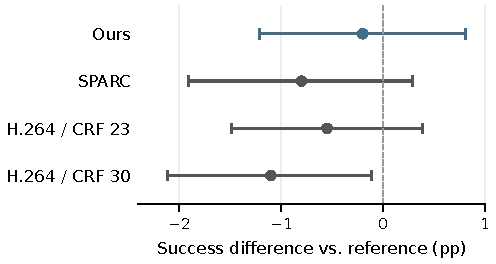
\includegraphics[width=\columnwidth]{images/libero-paired-differences.pdf}
\caption{Paired success-rate differences from the LIBERO reference.
Intervals are paired 95\% confidence intervals; they are not inferred
from independent binomial samples.}
\Description{A horizontal interval plot compares the proposed method,
SPARC, and two H.264 settings with the reference. The proposed method
has a difference of minus 0.20 percentage points with an interval
from minus 1.21 to plus 0.81.}
\label{fig:paired}
\end{figure}

SPARC had the smallest reported payload in this comparison. Our direct
success-rate difference from SPARC was $+0.60$ percentage points
($[-0.45,1.66]$, $p=0.299$). H.264 CRF 30 is below the reference by
$1.10$ percentage points ($[-2.11,-0.11]$, $p=0.035$), but the direct
comparison between our method and that H.264 setting is not significant.
The difference is $+0.90$ percentage points, with a 95\% interval of
$[-0.16,1.97]$ and $p=0.111$.
The stronger H.264 CRF 23 setting succeeded in 1,927 episodes at a larger
payload. These points characterize available operating configurations;
they do not establish a minimum bitrate required by either method.

Actual rANS deployment was checked on a separate 200-episode subset,
with 50 episodes per suite. Mean payloads were 1,857, 1,599, 2,035, and
1,787 bytes for Spatial, Object, Goal, and Long, respectively, giving
approximately 1.82\,kB per upload. The entropy path recovered the
quantized codes losslessly. Rerunning a policy can nevertheless change
individual episode outcomes, so coding correctness is distinguished
from rollout determinism.

\paragraph{RoboCasa input-domain sensitivity.}
Table~\ref{tab:robocasa} reports the first training-domain batch. The
reference succeeded in 291 episodes and the proposed configuration in
295, with a paired difference of $+0.83$ percentage points
($[-3.93,5.59]$, $p=0.797$). The second batch yielded 286 versus 275.
Pooling the two within-batch comparisons gives 577 reference successes
and 570 proposed-method successes in 960 episodes, a difference of
approximately $-0.7$ percentage points ($[-4.1,2.7]$, $p=0.72$).
The width of this interval prevents a narrow claim about preserved
performance.

\begin{table}[t]
\caption{First RoboCasa training-domain batch, 480 episodes. The
reference includes training-domain AV1 preprocessing but no extra
transport compression. Payloads are the recorded configuration summaries;
complete wire-level accounting is not established by this table.}
\label{tab:robocasa}
\centering\small
\begin{tabular}{lrr}
\toprule
Method & Payload (kB) & Successes \\
\midrule
Training-domain reference & -- & 291 \\
SPARC & 0.97 & 277 \\
H.264 CRF 44 & $\sim$1.1 & 4 \\
H.264 CRF 34 & $\sim$3.0 & 0 \\
Ours, lower rate & 1.14 & 295 \\
Ours, higher rate & 3.0 & 272 \\
\bottomrule
\end{tabular}
\end{table}

The reference itself changes with preprocessing: unprocessed 256
rendering gives 251 successes, and a separate native-224 protocol gives
190. We therefore do not interpret a comparison against the native-224
reference as a compression improvement under the training-domain
protocol. The low-rate H.264 configurations perform poorly in the first
batch, but available results do not establish a single causal source of
that failure or a complete high-rate recovery curve. Similarly, the
higher payload of one learned configuration does not ensure higher
success because these are separately trained operating points.

\subsection{Latency through the Deployed Stack}
The SO-101 latency experiment replays recorded red-block observations
through an Orin client and A40 policy server over the actual link.
Table~\ref{tab:replay} reports complete request quantiles and uses the
task-specific block checkpoint for SPARC. Both its original execution
layout and an all-GPU layout are included. Figure~\ref{fig:replay}
shows the corresponding median and 95th-percentile request times.

\begin{table}[t]
\caption{Recorded-observation replay through the deployed stack.
Each method has 195 uploads after warm-up. Payloads in this table
use KiB ($1\,\mathrm{KiB}=1,024$ bytes); SPARC payloads are in bytes.
These are request measurements, not physical task trials.}
\label{tab:replay}
\centering\small
\begin{tabular}{lrrr}
\toprule
Method & Payload & p50 (ms) & p95 (ms) \\
\midrule
Raw & 220.5 KiB & 397.1 & 815.6 \\
JPEG q90 & 15.2 KiB & 282.3 & 301.1 \\
H.264 CRF 30 & 1.2 KiB & 272.4 & 285.9 \\
SPARC block, original & 742 B & 856.3 & 933.1 \\
SPARC block, GPU & 742 B & 431.3 & 438.0 \\
Ours & 1.3 KiB & 228.4 & 237.5 \\
\bottomrule
\end{tabular}
\end{table}

\begin{figure}[t]
\centering
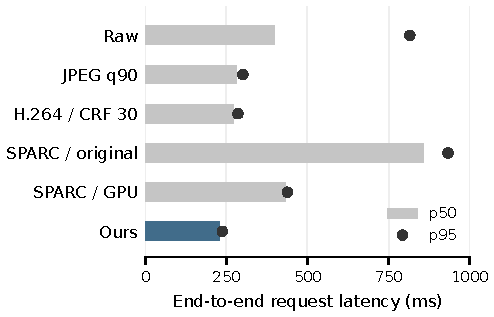
\includegraphics[width=\columnwidth]{images/replay-request-latency.pdf}
\caption{Complete request latency in recorded-observation replay.
Bars show p50 and points show p95; the point is a quantile, not an
uncertainty interval. SPARC uses the block-specific checkpoint.}
\Description{Horizontal latency bars and tail-quantile points for raw
images, JPEG, H.264, two SPARC execution layouts, and the proposed
feature path.}
\label{fig:replay}
\end{figure}

Median latency was 228.4\,ms for the proposed path and 272.4\,ms for
H.264, a reduction of approximately 16.2\% in this deployment.
The task-specific SPARC GPU layout had a smaller payload but a median
of 431.3\,ms. This comparison illustrates why payload and request
latency must be reported together. The ranking is not a result about
all cloud GPUs or networks.

The proposed path's edge median was 13.6\,ms, compared with 2.9\,ms for
H.264; its cloud-total median was 184.3\,ms versus 240.3\,ms. These are
separately aggregated stage measurements and do not add exactly to the
end-to-end medians. They identify the separate edge and cloud costs, while
the complete request duration remains the primary timing metric.
Uploads within a replay sequence are correlated, and no trial-level
confidence claim is derived from treating them as independent tasks.

\subsection{Backbone Adaptation and Component Diagnostics}
The initial OpenVLA-OFT evaluation covered 2,000 episodes, with
1,933 successes versus 1,923 for its reference. Subsequent evaluation
found baseline drift, motivating a contemporaneous rerun. The recorded
partial rerun contains 1,743 versus 1,748 successes in 1,800 episodes.
These windows are not pooled. Until the policy-matched SPARC and image
baselines are complete, this evidence supports interface feasibility
rather than a full cross-backbone compression ranking. The recorded
17.5\,kB OFT rate also requires consistent wire-level validation before
being compared with the primary configuration's sampled rANS payload.

A visual-path microbenchmark records 17.6\,ms for OFT edge encoding
and 10.2\,ms for cloud recovery. Its H.264 comparison includes 2.1\,ms
of edge encoding, 5.3\,ms of decoding, and 39.6\,ms for the original
visual towers. These component measurements use synthetic motion
frames for video decoding and are not a substitute for a complete
same-input deployment comparison.

For $\pi_{0.5}$, a recorded student-tower measurement is 11.0\,ms
versus 39.9\,ms for the original tower. The non-distilled codec variant
succeeds in 1,918 LIBERO episodes versus 1,934 for the main configuration.
This diagnostic does not isolate all effects of student training, codec
training, and runtime capture. The end-to-end encoding measurement in
Table~\ref{tab:replay} is therefore the appropriate deployment cost.
Likewise, the unquantized RoboCasa variant gives 290 successes versus
291 for its reference; this single operating point does not establish
that quantization is harmless across configurations.

\subsection{Distribution Shift and Current Coverage}
On the project's 700-episode LIBERO-Plus evaluation, the reference,
proposed method, and SPARC succeeded in 610, 590, and 558 episodes,
respectively. The proposed method is below its reference by approximately
2.9 percentage points ($p=0.047$), with deficits concentrated in camera
viewpoint and background texture. Its direct comparison with SPARC has
$p=0.004$. The positive comparison with SPARC does not remove the
degradation relative to the original policy.

The current evaluation does not establish physical closed-loop success,
energy per completed task, sustained thermal behavior, or recovery from
reference-state loss. The available bandwidth and stream-count tables
are analytical estimates under assumed service and network conditions;
they are not measured multi-robot experiments and are not used here as
deployment results.

\section{Discussion and Limitations}
\label{sec:limitations}
\paragraph{The advantage depends on the operating point.}
Direct token recovery removes receiver work but adds a light vision encoder
and feature codec to the robot. Its usefulness depends on the hardware,
network, and quality requirement. SPARC's smaller payload in the LIBERO
comparison is a real alternative, and H.264 can have lower computation
cost on a stronger cloud platform. The observed Orin-to-A40 latency
reduction should therefore be read as a deployment result, not a claim
that feature streaming dominates image transport everywhere. The
recorded $\pi_{0.5}$ concurrency experiment improves throughput by only
3--5\%, consistent with policy computation remaining a substantial cost
after visual encoding is removed.

\paragraph{Policy alignment is not a robustness guarantee.}
Training against the original policy constrains behavior on the training
distribution. It does not ensure that the recovered representation
preserves unfamiliar observations. The LIBERO-Plus result exposes this
boundary. An additional recorded Lego-policy diagnostic also gives
greater offline action deviation for the learned path than for JPEG.
Action deviation itself is not physical task success, but this negative
result prevents generalizing favorable red-block diagnostics to every
real-world policy. Adaptation to perturbed observations and prospective
physical trials are needed to characterize this boundary.

\paragraph{State and evaluation completeness.}
Conditional temporal coding assumes a consistent discrete reference. Integer
entropy coding verifies symbol recovery under that assumption; it does
not establish a recovery protocol under message loss or restart. The
codec is also trained separately for each policy interface, with a
training cost not fully characterized by the present measurements.
Finally, replay isolates a deployed inference path from physical
execution. Establishing a control benefit requires task trials that
record outcome and observation age together, with controlled resets
and a predefined statistical protocol.

\section{Related Work}
\label{sec:related}
\paragraph{Task-aware visual communication.}
Learned image compression jointly models a latent representation and its
coding distribution; scale hyperpriors are a representative
approach~\cite{hyperprior}. LimitNet studies progressive content-aware
offloading for constrained devices and networks~\cite{limitnet}.
For VLA policies, SPARC trains an image reconstruction path using action
distortion, temporal masking, and a tilted rate penalty~\cite{sparc}.
Our work shares the task-oriented objective but recovers policy features
rather than images. Action awareness itself is not the distinguishing
claim; the communication interface and its division of computation are.

\paragraph{Collaborative inference and feature compression.}
Neurosurgeon studies partitioning inference between a mobile device and
the cloud~\cite{neurosurgeon}. BottleNet++ explicitly compresses
intermediate features for device--edge inference~\cite{bottlenetpp}.
RoboECC and RAPID extend collaborative deployment and partitioned
inference to VLA models~\cite{roboecc,rapid}. Our contribution is not
model splitting or activation transmission alone. We combine a compact policy-supervised visual path
with quantized temporal state and a concrete entropy-coded interface;
a controlled comparison with simple feature quantization remains part
of the evaluation needed to attribute its gains.

\paragraph{VLA interfaces and timely execution.}
OpenVLA and $\pi_{0.5}$ provide the policy families underlying our
implementation~\cite{openvla,pi05}. OpenVLA-OFT studies adaptation,
continuous action prediction, and action chunking~\cite{openvlaoft}.
Our method freezes the associated policy and changes its visual
input path. Distillation supplies the general teacher--student
principle~\cite{distillation}, while the per-policy visual interface
determines what representation the receiver must reconstruct.

ARIA studies inference across heterogeneous mobile
processors~\cite{aria}, and TimelyLLM coordinates generation with
physical agent execution~\cite{timelyllm}. Their settings reinforce
the need to relate compute timing to application behavior. The current
system uses existing asynchronous execution; its contribution concerns
visual representation and transmission rather than a new scheduling
algorithm.

\section{Conclusion}
\label{sec:conclusion}
We presented a feature-streaming interface for edge--cloud VLA inference.
A distilled edge tower and learned codec produce a quantized temporal
bitstream, and the cloud recovers inputs to a frozen policy without
first reconstructing images. Quantized reference state avoids a neural
decoder on the robot. The available simulation and deployment-replay
results show a useful quality--cost operating point for the primary
configuration, while also exposing smaller-payload alternatives,
distribution-shift losses, and deployment-dependent timing benefits.
Further physical trials, matched feature-transfer baselines, and
complete training and wire-level measurements are required to determine
how broadly this interface improves robotic operation.

\begin{thebibliography}{18}
\bibitem{pi05}
Physical Intelligence et al. 2025.
$\pi_{0.5}$: a Vision-Language-Action Model with Open-World Generalization.
arXiv:2504.16054. \url{https://arxiv.org/abs/2504.16054}.
\bibitem{openvla}
Moo Jin Kim, Karl Pertsch, Siddharth Karamcheti, et al. 2025.
OpenVLA: An Open-Source Vision-Language-Action Model.
In \emph{Proceedings of the 8th Conference on Robot Learning},
PMLR 270, 2679--2713.
\url{https://proceedings.mlr.press/v270/kim25c.html}.
\bibitem{openvlaoft}
Moo Jin Kim, Chelsea Finn, and Percy Liang. 2025.
Fine-Tuning Vision-Language-Action Models: Optimizing Speed and Success.
In \emph{Robotics: Science and Systems XXI}.
\url{https://doi.org/10.15607/RSS.2025.XXI.017}.
\bibitem{limitnet}
Ali Hojjat, Janek Haberer, Tayyaba Zainab, et al. 2024.
LimitNet: Progressive, Content-Aware Image Offloading for Extremely Weak
Devices \& Networks.
In \emph{MobiSys}, 519--533.
\url{https://doi.org/10.1145/3643832.3661856}.
\bibitem{sparc}
Hyeonjun Kim, Jegwang Ryu, Sangbeom Ha, et al. 2026.
Learned Image Compression for Vision-Language-Action Models.
arXiv:2606.16253v2.
\url{https://arxiv.org/abs/2606.16253v2}.
\bibitem{neurosurgeon}
Yiping Kang, Johann Hauswald, Cao Gao, et al. 2017.
Neurosurgeon: Collaborative Intelligence Between the Cloud and Mobile Edge.
In \emph{ASPLOS}, 615--629.
\url{https://doi.org/10.1145/3037697.3037698}.
\bibitem{roboecc}
Zihao Zheng, Hangyu Cao, Jiayu Chen, et al. 2026.
RoboECC: Multi-Factor-Aware Edge-Cloud Collaborative Deployment for VLA Models.
arXiv:2603.20711.
\url{https://arxiv.org/abs/2603.20711}.
\bibitem{rapid}
Zihao Zheng, Sicheng Tian, Hangyu Cao, et al. 2026.
RAPID: Redundancy-Aware and Compatibility-Optimal Edge-Cloud Partitioned
Inference for Diverse VLA Models.
arXiv:2603.07949.
\url{https://arxiv.org/abs/2603.07949}.
\bibitem{bottlenetpp}
Jiawei Shao and Jun Zhang. 2020.
BottleNet++: An End-to-End Approach for Feature Compression in
Device-Edge Co-Inference Systems.
In \emph{IEEE ICC Workshops}.
\url{https://doi.org/10.1109/ICCWorkshops49005.2020.9145068}.
\bibitem{distillation}
Geoffrey Hinton, Oriol Vinyals, and Jeff Dean. 2015.
Distilling the Knowledge in a Neural Network.
arXiv:1503.02531.
\url{https://arxiv.org/abs/1503.02531}.
\bibitem{ans}
Jarek Duda. 2013.
Asymmetric numeral systems: entropy coding combining speed of Huffman
coding with compression rate of arithmetic coding.
arXiv:1311.2540.
\url{https://arxiv.org/abs/1311.2540}.
\bibitem{timelyllm}
Neiwen Ling, Guojun Chen, Anurag Khandelwal, et al. 2026.
TimelyLLM: Time-sensitive LLM Serving System for Physical-I/O Limited Agents.
In \emph{MobiSys}.
\url{https://doi.org/10.1145/3745756.3809203}.
\bibitem{hyperprior}
Johannes Ball\'e, David Minnen, Saurabh Singh, et al. 2018.
Variational Image Compression with a Scale Hyperprior.
In \emph{ICLR}.
\url{https://arxiv.org/abs/1802.01436}.
\bibitem{siglip}
Xiaohua Zhai, Basil Mustafa, Alexander Kolesnikov, et al. 2023.
Sigmoid Loss for Language Image Pre-Training.
In \emph{ICCV}, 11975--11986.
\url{https://openaccess.thecvf.com/content/ICCV2023/html/Zhai_Sigmoid_Loss_for_Language_Image_Pre-Training_ICCV_2023_paper.html}.
\bibitem{dinov2}
Maxime Oquab, Timoth\'ee Darcet, Th\'eo Moutakanni, et al. 2023.
DINOv2: Learning Robust Visual Features without Supervision.
arXiv:2304.07193.
\url{https://arxiv.org/abs/2304.07193}.
\bibitem{libero}
Bo Liu, Yifeng Zhu, Chongkai Gao, et al. 2023.
LIBERO: Benchmarking Knowledge Transfer for Lifelong Robot Learning.
In \emph{Advances in Neural Information Processing Systems 36},
Datasets and Benchmarks Track.
\url{https://arxiv.org/abs/2306.03310}.
\bibitem{robocasa365}
Soroush Nasiriany, Sepehr Nasiriany, Abhiram Maddukuri, et al. 2026.
RoboCasa365: A Large-Scale Simulation Framework for Training and
Benchmarking Generalist Robots.
In \emph{ICLR}.
\url{https://arxiv.org/abs/2603.04356}.
\bibitem{aria}
Chanyoung Jung, Jeho Lee, Gunjoong Kim, et al. 2025.
ARIA: Optimizing Vision Foundation Model Inference on Heterogeneous
Mobile Processors for Augmented Reality.
In \emph{MobiSys}.
\url{https://doi.org/10.1145/3711875.3729161}.
\end{thebibliography}

\appendix
\section{Additional Evaluation Context}
\label{app:context}
\subsection{Evaluation Units and Pairing}
The main LIBERO comparison contains 2,000 episodes per method: four
suites, ten tasks per suite, and 50 episodes per task. Outcomes are paired
by initial state within the same evaluation framework and host. The
success-rate difference is reported as method minus reference in
percentage points. The paired confidence intervals and exact two-sided
McNemar tests use the discordant outcomes, that is, episodes in which
only one member of a pair succeeds. A test against the reference and a
direct test between two compressed methods answer different questions;
one method's significant difference from the reference does not establish
a significant difference between the two methods.

The 200-episode rANS deployment check is a separate sample, with 50
episodes per suite. Its payload measurements are associated with the
primary configuration but do not establish that all 2,000 success-rate
episodes traversed the deployed entropy-coding path. Episode counts,
payload samples, and upload timing samples therefore retain separate
denominators throughout the evaluation.

\subsection{Input Protocols and Evaluation Windows}
The RoboCasa input protocol is part of the experiment definition.
Native 224 rendering, unprocessed 256 rendering, and training-domain AV1
processing produce different inputs to the same policy. Their reference
success rates are not interchangeable. The comparison in
Table~\ref{tab:robocasa} uses the training-domain protocol; the pooled
reference and proposed-method result combines two batches, with
comparisons matched within each batch and host.

Each RoboCasa batch contains 24 tasks and 20 episodes per task. The first
batch ran on A100 and the second on A40; their reference and proposed
method counts were 291 versus 295 and 286 versus 275, respectively.
The pooled 960-episode result combines the paired comparisons within
these batches. It does not pair outcomes across hosts. In the first
batch, the reference, SPARC, and H.264 clients shared a policy service,
so matching initial states did not align the policy's random-number
sequence for every invocation.

OpenVLA-OFT results also belong to distinct evaluation windows. The
initial complete window and the partial contemporaneous rerun are
reported independently because the reference policy exhibited drift.
A codec trained for another backbone is a transfer diagnostic rather
than a policy-matched primary baseline.

\subsection{Perturbation Breakdown}
Table~\ref{tab:appendix-perturbations} gives the category counts behind
the 700-episode LIBERO-Plus result. Each category contains 100 episodes.
The proposed codec was trained on the original LIBERO observations.
Its largest observed deficits relative to the reference were nine
successes under camera-viewpoint changes and seven under background
texture changes. The table describes where the observed deficit occurs;
it does not isolate its cause. Individual category counts also do not
establish a general robustness ranking across policies or perturbation
distributions.

\begin{table}[t]
\caption{LIBERO-Plus successes by perturbation category. Each category
has 100 paired episodes. The total row covers 700 episodes per method.}
\label{tab:appendix-perturbations}
\centering\small
\setlength{\tabcolsep}{4pt}
\begin{tabularx}{\columnwidth}{Xrrr}
\toprule
Perturbation & Reference & Ours & SPARC \\
\midrule
Camera viewpoint & 85 & 76 & 76 \\
Background texture & 96 & 89 & 83 \\
Language instruction & 93 & 89 & 92 \\
Lighting & 94 & 96 & 83 \\
Object layout & 84 & 85 & 83 \\
Robot initial state & 78 & 76 & 67 \\
Sensor noise & 80 & 79 & 74 \\
\midrule
Total & 610 & 590 & 558 \\
\bottomrule
\end{tabularx}
\end{table}

\section{Measurement Scope}
\label{app:measurement}
\subsection{Payload Accounting}
The LIBERO rANS subset yielded mean payloads of 1,857, 1,599, 2,035,
and 1,787 bytes per upload for Spatial, Object, Goal, and Long,
respectively. These measurements cover both camera streams. The
reported summary is approximately 1.82\,kB per upload; its scope is
codec payload rather than complete network traffic.

For SO-101 replay, the reporting script averages the per-upload
\texttt{payload\_bytes} field after warm-up. It divides values of at
least 1,024 bytes by 1,024 for display. Table~\ref{tab:replay} labels
these values as KiB and retains bytes for the smaller SPARC payloads.
This unit convention is distinct from the simulation summaries.

\subsection{Timing and Aggregation}
The replay discards the first five of 200 uploads for each method,
leaving 195 uploads. For each timing field, the reporting script sorts
the available values and selects the element at the nearest integer
index to the requested fraction of the zero-based index range. It does
not interpolate between adjacent observations. With 195 valid values,
p50 and p95 are the 98th and 185th sorted observations, respectively.
These are empirical upload quantiles rather than confidence limits.

Cloud-total time includes cloud decoding and policy computation; for
image paths, it also includes the original visual encoder. Cloud
decoding is therefore already included in cloud-total time. The network
residual subtracts edge encoding and cloud-total time from the complete
request duration, retaining transfer, response return, and serialization
effects. It is not a separately timed one-way network delay.

End-to-end quantiles are computed from complete request measurements.
Summing stage medians would generally combine values from different
uploads and does not recover the median request duration. Likewise,
synchronized component microbenchmarks and the captured deployed path
have different timing boundaries, as described in
\S\ref{sec:implementation}.

\subsection{Physical Interpretation}
The replay experiment uses recorded observations without corresponding
physical task execution. It can characterize request processing under
the measured trace but cannot quantify recovery from an execution error,
success under moving objects, or the age of an observation when a
physical actuator applies the returned action.

\section{Use of Generative Writing Assistance}
Generative AI assisted in drafting and editing the manuscript text and
in preparing an initial architecture illustration. The experimental
results are drawn from the project's recorded summaries; the writing
process did not generate or rerun those experiments.

\end{document}
